Consider a binary system of black holes, both of equal mass $M$, separated by a distance $a$, and revolving around their common center of mass (CM) in circular orbits. This binary system moves against, and interacts with, a very large, uniform field of stars (each of mass $m \ll M$) with number density $n$. Consider a star that approaches the system from infinity with speed $v$ and impact parameter $b$, in the reference frame of the CM (as shown in the figure below). Its closest approach distance to the CM is $r_p \approx \frac{1}{2}a$. For tasks (a) and (c), you should make use of the fact that $v^2 \ll \frac{GM}{a}$.


\begin{figure}[h!]
    \centering    
    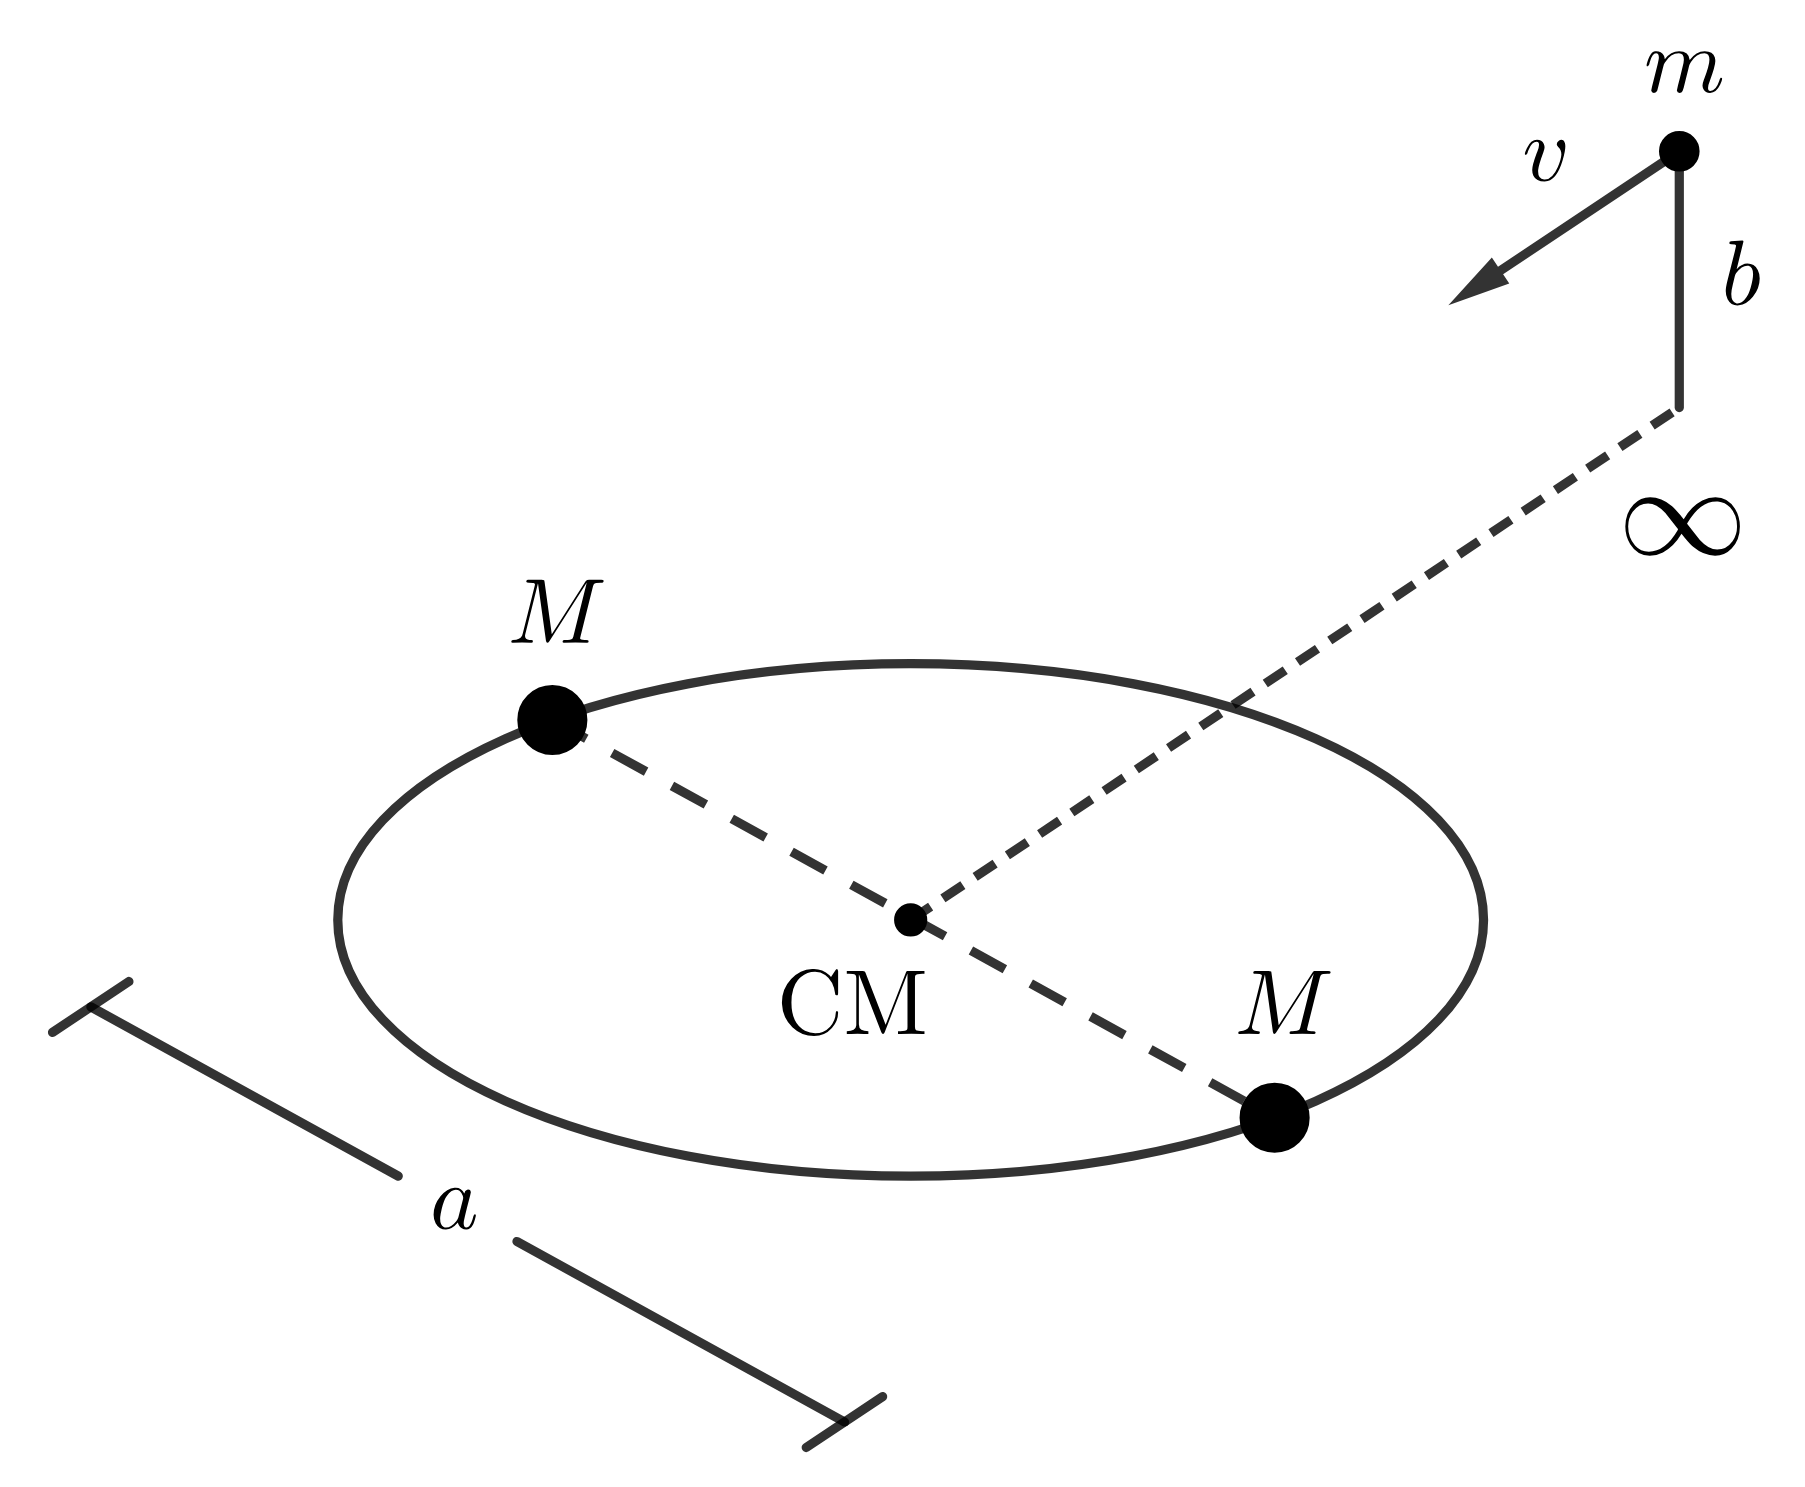
\includegraphics[scale=0.3]{2024/Theory/Figures/2024_TH_Q8_F1.png}
    \caption{Diagram of the system}
    \label{fig:binary1}
\end{figure}

\begin{parts}
    \part[5] Obtain an expression for $b$, in terms of $M$, $a$, $v$, and physical constants. In this task, assume that the star interacts with the binary as if its total mass was fixed at the CM.

    \uplevel{After a complex interaction with the binary, the star is slingshot from the system. The exact calculation of its ejection speed is complex, but the result can be estimated by considering that the star only interacts with one of the components when near the system. As such, consider, in part (b), \textit{only} the gravitational interaction between the star and \textit{one of the components} in the binary.}
    
    \part[6] The star approaches the component with an initial speed negligible compared to the component's orbital speed, and both are moving directly towards each other. After interacting with the system, when the star is again far away from the black hole, we find that the direction of its velocity vector is reversed and the final speed is $v_f$. Determine $v_f$, in terms of $M$, $a$, $v$, and physical constants. Assume that linear momentum and mechanical energy are conserved during this interaction and that it takes place in a timescale much smaller than the binary's period. Recall that $m \ll M$.

    \uplevel{For the following task, assume that all stars approaching the system from infinity with an impact parameter $\frac{1}{2}b_{0} \leq b \leq \frac{3}{2}b_{0}$ (where $b_0$ is the impact parameter of a star whose speed at infinity is $v_{0}$) attain a closest-approach distance $r_p \approx \frac{1}{2}a$ to the CM. \textbf{Also assume that all stars exit the system with the speed found in (b).}}


    \part[14] Upon each encounter, part of the total energy of the binary is transferred to the kinetic energy of the star. Assume that the binary orbit remains circular. Knowing this, using your results from previous tasks, and taking into account only encounters with the stars within the specified range of impact parameters, show that the reciprocal of the binary's separation increases at a constant rate:
    \[\dfrac{\text{d} }{\text{d} t} \left(\dfrac{1}{a}\right) = H \dfrac{G\rho}{v_{0}}\]
    Here, $\rho = nm$ is the mass density of the star field, and $G$ the universal gravitational constant. Find the dimensionless constant $H$, which refers to hardening.
\end{parts}